\documentclass[a4paper,UTF8]{article}
\usepackage{ctex}
\usepackage[margin=1.25in]{geometry}
\usepackage{color}
\usepackage{graphicx}
\usepackage{amssymb}
\usepackage{amsmath}
\usepackage{amsthm}
%\usepackage[thmmarks, amsmath, thref]{ntheorem}
\theoremstyle{definition}
\newtheorem*{solution}{Solution}
\newtheorem*{prove}{Proof}
\usepackage{multirow}
\usepackage{url}
\usepackage[colorlinks,urlcolor=blue]{hyperref}
\usepackage{enumerate}
\renewcommand\refname{参考文献}


%--

%--
\begin{document}
\title{\textbf{《计算机图形学》3月报告}}
\author{211240045,杨镇源,\href{mailto:211240045@smail.nju.edu.cn}{211240045@smail.nju.edu.cn}}
\maketitle

\section{综述}

\subsection{2024年3月}

\subsubsection{cg\_algorithms.py}

$\bullet$ 完成绘制直线(DDA算法)

$\bullet$ 完成绘制直线(Bresenham算法)

\subsubsection{cg\_gui.py}

$\bullet$ 实现gui重置画布

$\bullet$ 实现gui保存画布

\subsection{2024年4月}

\subsubsection{cg\_algorithms.py}

$\bullet$ 完成绘制多边形(DDA算法)

$\bullet$ 完成绘制多边形(Bresenham算法)

$\bullet$ 完成绘制椭圆(中点圆生成算法)

$\bullet$ 完成图元平移

\subsubsection{cg\_gui.py}

$\bullet$ 实现gui设置画笔颜色

\section{算法介绍}

\subsection{绘制直线}

\subsubsection{DDA算法}

\textbf{算法原理:}DDA算法的核心思想是通过计算斜率来确定每个像素点的位置,从而形成一条连续的直线。通过坐标轴上以单位间隔取样($\Delta x = 1$或$\Delta y = 1$),因为取单位间隔,所以显见对应的$\Delta y = k, -k$或$\Delta x = \frac{1}{k},-\frac{1}{k}$(记直线为$y=kx+b$)。当起始点在左侧取值,起始点在右侧取负值。

\textbf{算法改进:}可利用直线构成的连贯性,通过将增量$k$和$\frac{1}{k}$分离成整数和小数部分从而使所有的计算都简化为整数操作来改善DDA算法的性能。

\subsubsection{Bresenham算法}

\textbf{算法原理:}通过坐标轴上以单位间隔取样($\Delta x = 1$或$\Delta y = 1$),不失一般性取$0\leq k<1$。假设$(x_k,y_k)$为已经确定的像素坐标,那么下一个像素坐标为$(x_{k}+1,y_k)$或$(x_k+1,y_k+1)$,确定$y$轴坐标选择哪一个的依据是判断直线和$x=x_k+1$的交点的$y$轴坐标与$y_k+1,y_k$哪个的绝对差值更小。若与$y_k$绝对差值更小,则下一个点选择$(x_k+1,y_k)$;若与$y_k+1$绝对差值更小,则下一个点选择$(x_k+1,y_k+1)$。

\textbf{算法改进:}为进一步提高算法效率,可以利用线段本身的对称性。用Bresenham算法产生起点一侧的半条线段,至于终点一侧的半条线段,可以看作以终点为起点线段的生成。起点一侧的线段像素坐标在$x$或$y$方向每前进一个坐标单位,终点一侧的线段像素坐标就在$x$或$y$方向后退一个坐标单位。

\subsubsection{方法对比}

DDA算法的优点在于适用面广,实现简单。但是它存在一个问题,在计算斜率时会产生精度损失,从而使得绘制出来的直线可能出现明显的锯齿状。因此,在对线条的精度有较高要求的情况下,可以采用Bresenham算法。

Bresenham算法通过整数计算来绘制线条,避免了DDA算法中的精度损失问题。因此,Bresenham算法具有更高的绘制速度和较好的像素级别的控制,可以在需要绘制直线的情况下带来更好的性能和画质。

总的来说,Bresenham算法比DDA算法绘制直线更准确高效。

\subsection{绘制多边形}

绘制多边形的方法基于绘制直线的算法,对于多边形的每条边,获得其两端点后利用直线绘制算法进行绘制即可。

\subsection{绘制椭圆}

\subsubsection{中心椭圆生成算法}

\textbf{算法原理:}算法类似于Bresenham算法,不失一般性,考虑中心在原点处的椭圆,研究第一象限。将第一象限中椭圆切线绝对值等于1所对应的切点记作临界点$P$,$P$上方的点$\frac{dy}{dx}<1$,$P$下方的点$\frac{dy}{dx}>1$,由此可利用Bresenham算法解决选点问题。根据参数方程定义椭圆函数为:
$$f_{ellipse}(x,y)=b^2x^2+a^2y^2-a^2b^2$$
在$P$上方的点,取$x$方向单位步长,再通过决策函数判断真实值与两候选像素之间哪个位置
更近,更新对应的$y$值;在$P$下方的点,取$y$方向单位步长,再通过决策函数判断真实值与两候选像素之间哪个位置
更近,更新对应的$x$值。又因为椭圆四个象限是互相对称的,可以通过改变对应的符
号补全其余象限,最后结合中心点的实际坐标即可计算出待绘制椭圆的点坐标。
\section{系统介绍}

\subsection{图元平移}

需要实现或改动的函数有:

$\bullet$ start\_translate函数

$\bullet$ mousePressEvent函数

$\bullet$ mouseMoveEvent函数

$\bullet$ mouseReleaseEvent函数

$\bullet$ MainWindow类中连接槽函数,实现translate\_action函数

在start\_translate函数将当前系统状态调整为translate;在mousePressEvent函数中确定平移对象并记录初始位置;在mouseMoveEvent函数中随着鼠标指针移动,调用alg.translate函数更新平移对象的点集坐标,然后刷新界面。由此,即可完成平移功能。

\subsection{gui重置画布}

实现reset\_canvas\_action函数即可:

$\bullet$ 将所有画好的图形都删掉,并且将各参数重置为初始值

$\bullet$ 通过QDialog获取并记录新设置的宽和高

$\bullet$ 将画布的宽和高设置为Dialog中得到的宽和高

\subsection{gui保存画布}

\subsection{gui设置画笔颜色}

1. 首先实现set\_pen\_action函数:

$\bullet$调用QColorDialog类中的getColor函数获得新的颜色值

$\bullet$将颜色值存入画布的temp\_color成员中

2. 后在MyCanvas类中创建新的图形Item时,将temp\_color作为参数传入构造函数,初始化图形Item的color成员

3. 调用painter.drawPoint函数画图前,使用setPen函数设置画笔颜色,保证图形颜色符合预期

效果如下图:

\begin{center}
	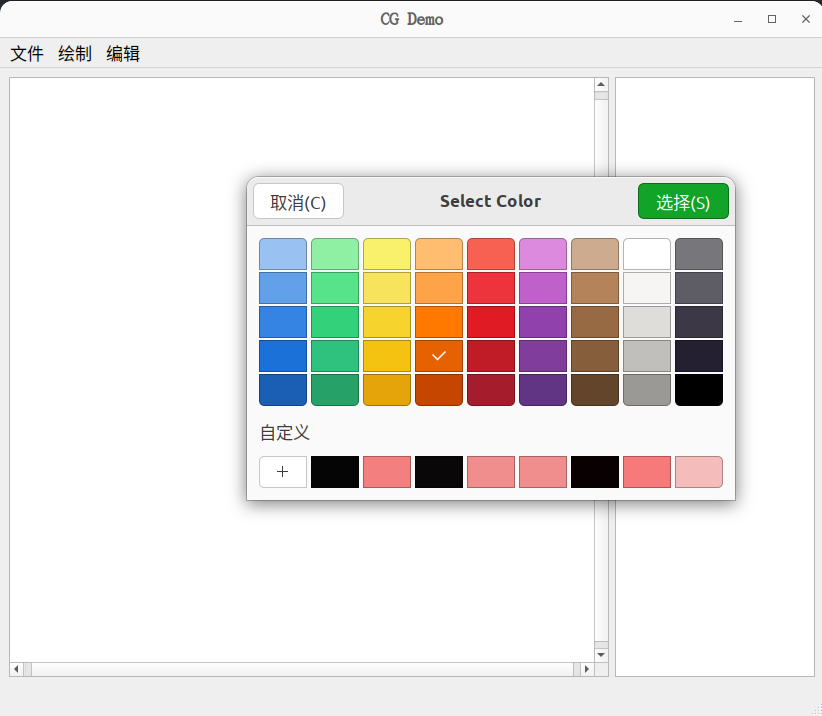
\includegraphics[width=6in]{figs/color1.png}
	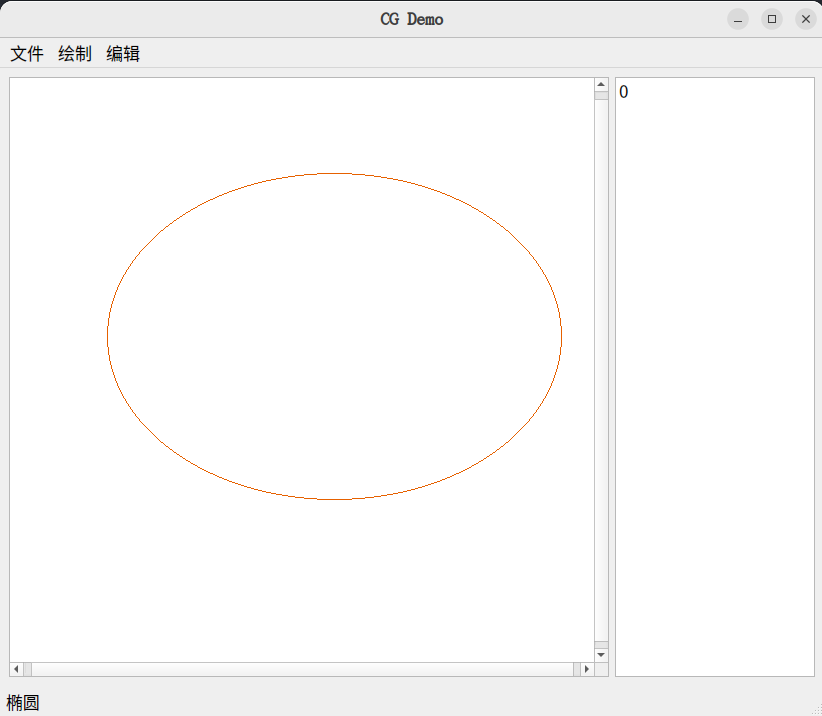
\includegraphics[width=6in]{figs/color2.png}
\end{center}

\section{总结}
\dots

\bibliographystyle{plain}%
%"xxx" should be your citing file's name.
\bibliography{xxx}

\end{document}